\section{Device Assembly} \label{sec:device_assebly}

\subsection{PCB Assembly}
The assembly process begins with the population of the \ac{PCB}.
To create a stable, level surface for applying solder paste, a jig made from spare boards is recommended.
Once the stencil is aligned, solder paste is applied evenly across the pads.
Next, the \ac{SMD} components are carefully placed using tweezers, with the exception of the \ac{MCU}, which is installed later.
The board is then reflowed using a heating plate or oven.

\begin{figure}[H]
	\centering
	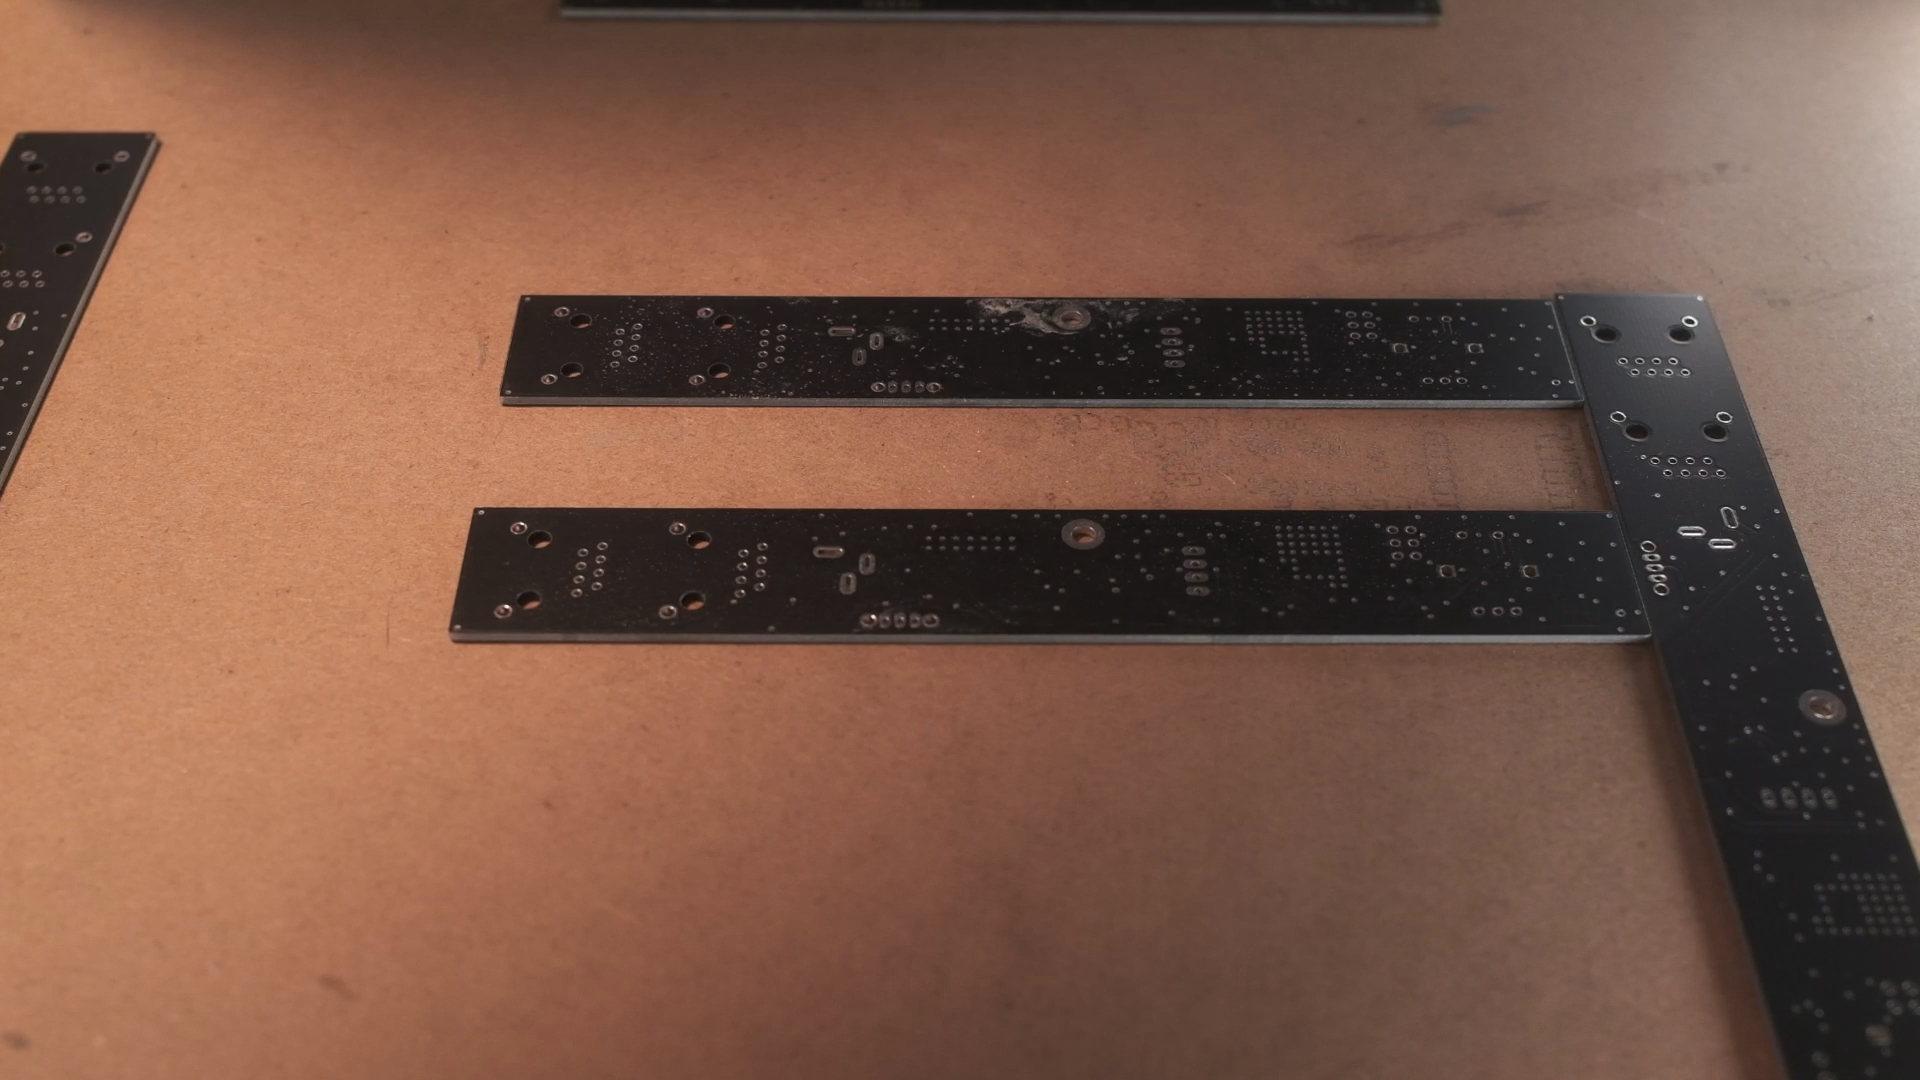
\includegraphics[width=0.8\linewidth]{graphics/pcb_jig}
	\caption{Assembly jig of the PCB}
	\label{fig:pcb_assembly}
\end{figure}

After the reflow process, the \ac{DC} jack is soldered manually.
Before proceeding with sensitive components, a 24V power source is connected to verify the 5V regulator's output with a multimeter; ensuring a stable voltage here is critical.
Once verified, the remaining \ac{THT} components, including the \ac{MCU} and pin headers, are soldered.
Special care should be taken to align the display's pin header at a precise 90-degree angle.
Finally, flux residues are cleaned using \ac{IPA}, and the \ac{LED} strip is prepared by cutting it to one-meter segments and desoldering any factory-installed wires.

\subsection{Firmware Configuration and Flashing}
To configure the software, download the firmware source code from the project repository and open it in the Arduino \ac{IDE}.
Ensure the Espressif board manager \ac{URL} is added to the preferences, then install the ESP32 board package (Version 3.30.3) via the Boards Manager.
Select \texttt{XIAO\_ESP32C3} as the target board.
Before flashing, adjust any necessary configuration parameters, such as the pixel count, in \texttt{config.h}.
Connect the board via \ac{USB}-C and upload the firmware; a successful flash is confirmed by the "Done uploading" message in the console.

\subsection{Mechanical Assembly}
\subsubsection{Preparation}
The enclosure components—including the housing bottom, top part, endcaps, and rotary encoder knob—are fabricated using \ac{FDM} printing.
M3 threaded inserts are then installed into the bottom housing and endcaps using a soldering iron, ensuring they sit flush with the surface.
The aluminum profile is cut into two one-meter sections.
Using the provided drill template, mounting points are marked with a center punch and drilled using a 3.5 mm bit.

\subsubsection{Wiring and Integration}
Wires are prepared as follows:
\begin{itemize}
	\item Data: 15 cm, 20 \ac{AWG}
	\item Power: 5 cm, 18 \ac{AWG}
\end{itemize}
Pre-tin the wire ends and solder them to the \ac{LED} strip.
The \ac{OLED} display is then attached to the \ac{PCB} using a spacer and double-sided tape for alignment. \\

Secure the end caps and bottom housing to the aluminum profile using M3 bolts, and mount the \ac{PCB} to the bottom housing using two 8 mm standoffs.
Install the \ac{LED} strip into the profile, routing the data line through a cable clip for a clean look.
Feed the wires through to the rear, strip the insulation, and solder them to the corresponding \ac{PCB} pads. \\

Install the antenna into the top housing and connect it to the ESP32, ensuring it does not interfere with the onboard buttons.
Secure the top cover to the standoffs and press the 3D-printed knob onto the rotary encoder shaft.
To finish the assembly, slide the diffuser under the endcaps and snap it into place.
